\documentclass[custom]{linearbook}

% 字体接口
%--------------------------------------------------------------------------
% 标题字体
\newcommand{\titlefont}{\CJKfontspec[AutoFakeBold=true]{方正清刻本悦宋简体.ttf}}
% 页眉字体
\newcommand{\headfont}{\CJKfontspec[AutoFakeBold=true]{方正楷体简体}}
% 黑体加粗
\newcommand{\blackheavy}{\CJKfontspec[AutoFakeBold=true]{方正黑体_GBK}}


\begin{document}
% 将XITS中的\pi和\sum替换为Computer Modern Math中对应的符号,可取消
%--------------------------------------------------------------------------
\let\pi\mpi
\let\sum\msum

% \pagestyle{fancy}
\pagenumbering{Alph}
% 封面
%--------------------------------------------------------------------------
\bookmark[page=1, level=1]{封面}
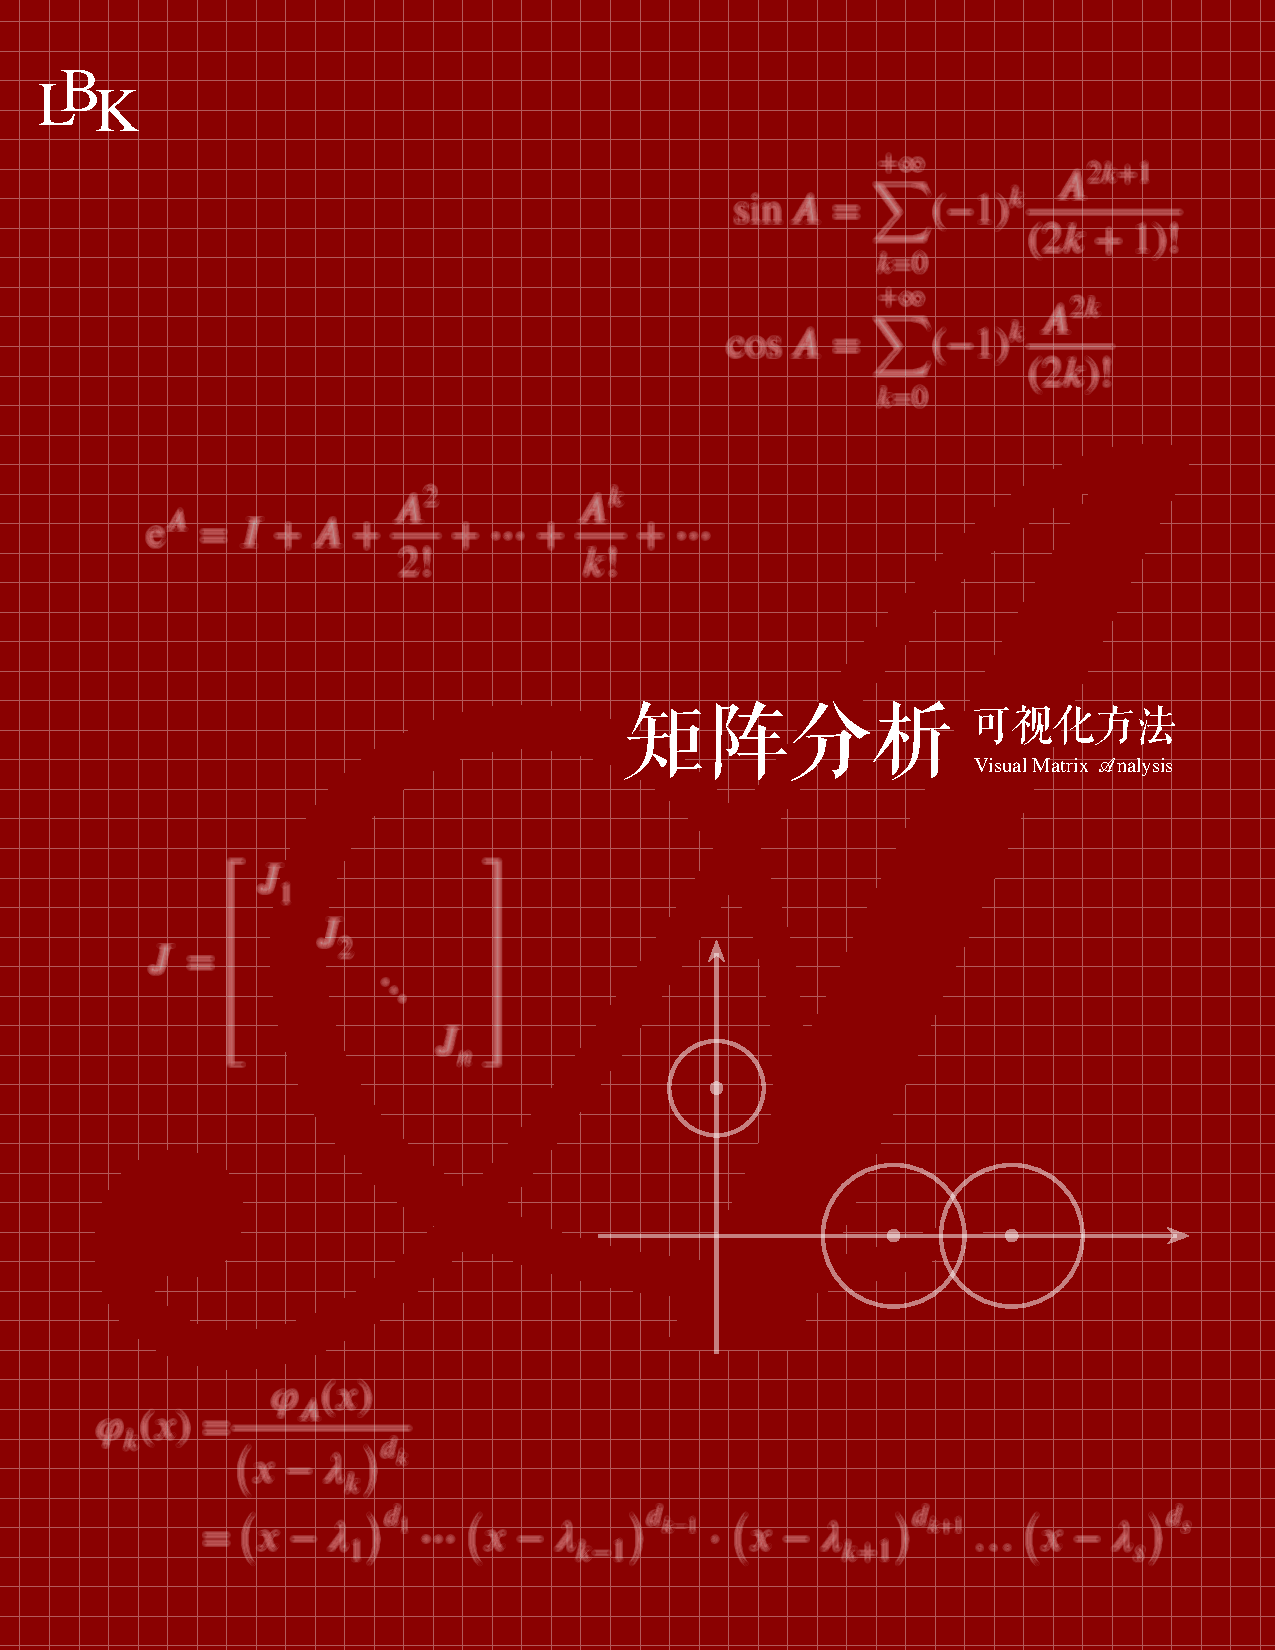
\includepdf[noautoscale=true, width=\paperwidth]{cover_backcover/cover.pdf}  % 先编译好,作为pdf插入

\frontmatter
\setcounter{page}{1}
\fancyhf{}
\pagestyle{other}

% 扉页
%--------------------------------------------------------------------------
\newpage
\newgeometry{includemp=true,
             inner=2cm,outer=2cm,
             top=2cm,bottom=1.5cm,
             headsep=0.5cm,headheight=0.5cm,
             footskip=0.7cm,
             marginparsep=0cm,marginparwidth=0cm}
\thispagestyle{empty}
\bookmark[page=3, level=1]{扉页}

\begin{tikzpicture}[remember picture,overlay]
    \node at (current page.north west)
      {
        \begin{tikzpicture}[remember picture,overlay]
          \draw[fill=lbdeepblue,draw opacity=0]
            ++(0,-2cm) rectangle ++(\paperwidth,-4pt);
          \node[color=lbdeepblue] (text)
            at  (0.35\paperwidth,-0.25\paperheight)
            {\titlefont\fontsize{60}{60}\selectfont  矩阵分析};
          \node[color=lbdeepblue,above right] at ($(text.east)+(0em,-0.5em)$)
          {\titlefont\fontsize{30}{40}\selectfont 可视化方法};
          \node[color=lbgreen,below right] (V) at ($(text.east)+(0.2em,-1em)$) {\fontsize{15}{25}\selectfont{Visual Matrix\, {$\symscr{A}$}nalysis}};
          \draw[line width=2pt,color=lbgreen] 
            ++(2cm,-2cm) |- ($(V.south east)+(0,-1cm)$);
        \end{tikzpicture}
      };
\end{tikzpicture}

\vspace*{10cm}

\hspace{0.5em}\begin{minipage}{0.9\linewidth}
  \zihao{-2}

  \textit{A Sample of} \LBK : \texttt{linearbook.cls}. 
  
  \vspace{2cm}

  \textit{\zihao{-3} Designed by}
  
  J.Wang
\end{minipage}

\vfill
\begin{center}
  \zihao{4}
  \titlefont

  还\;不\;知\;道\;哪\;个\;出\;版\;社

  北\quad 京
\end{center}
\restoregeometry

% 版权页
%--------------------------------------------------------------------------
\newpage
\newgeometry{includemp=true,
             inner=2cm,outer=2cm,
             top=2cm,bottom=1.5cm,
             headsep=0.5cm,headheight=0.5cm,
             footskip=0.7cm,
             marginparsep=0cm,marginparwidth=0cm}
\thispagestyle{empty}
\bookmark[page=4, level=1]{版权页}

\centerline{\textbf{内容简介}}
\vspace{0.8em}
{
\zihao{-5}

本书比较全面、系统地介绍了矩阵的基本理论、方法及其应用,全书分上、下两篇,上篇为基础篇,下篇为应用篇,共8章,分别介绍了矩阵的几何理论(包括线性空间与线性算子,内积空间与等积变换),矩阵与若尔当标准形,矩阵的分解,赋范线性空间与矩阵范数,矩阵微积分及其应用,广义逆矩阵及其应用,儿类特殊矩阵与特殊积(如非负矩阵与正矩阵、循环矩阵与素矩阵、随机矩阵和双随机矩阵、单调矩阵、M矩阵与H矩阵、T矩阵与汉克尔矩阵以及克罗内克积、阿达马积与反积等),前7章每章均配有一定数量的习题.附录中还给出了15套模拟自测试题,所有习题和自测题(约1300题)的详细解答,即将由清华大学出版社另行出版.

本书可作为理工科大学各专业研究生的学位课程教材,也可作为理工科和师范类院校高年级本科生的选修课教材,并可供有关专业的教师和工程技术人员参考.

\vfill

\noindent\hc{版权所有,侵权必究.}

\vspace{2em}

\begin{minipage}{0.9\linewidth}
    \hc{图书在版编目(CIP)数据}

    \vspace{1em}

    矩阵分析:可视化方法 / J. Wang编著. —北京:还不知道哪个出版社, 2222

    ISBN 996-7-618-12345-7

    \Romannum{1}.\ding{172}矩… \quad \Romannum{2}.\ding{172}Wang… \quad \Romannum{3}.\ding{172}矩阵分析 \quad \Romannum{4}. \ding{172}O151.7$x$ \quad 

    中国版本图书馆CIP数据核字(2222)第777777号
\end{minipage}

\vfill

\noindent\hc{责任编辑:} 阿\quad 磊\quad 陈尼龙 \par
\noindent\hc{封面设计:} J. Wang \par
\noindent\hc{责任校对:} 李涤纶 \par
\noindent\hc{责任印制:} 谢纯棉

\vspace{2em}
\noindent\hc{出版发行:} 还不知道哪个出版社

\vspace{0.5em}
\noindent\sj[4.7]\begin{minipage}{0.8\linewidth}
    \hc{网\qquad 址:} \texttt{http://www.hbzd.press.cn}  \par
    \hc{地\qquad 址:} 北京还不知道那条路66号A座 \qquad \hc{邮\qquad 编:} 000000 \par
    \hc{投稿与读者服务:}    \par
    \hc{质量反馈:}         
\end{minipage}

\vspace{0.5em}
\noindent\hc{印\qquad 刷:} \par
\noindent\hc{装\qquad 订:} \par
\noindent\hc{经\qquad 销:} \par
\noindent\hc{开\qquad 本:} 8\,\si{in}$\times$10\,\si{in}\qquad \hc{印\qquad 张:} 27.7 \qquad \hc{字\qquad 数:}  777千字\par
\noindent\hc{版\qquad 次:} 2222年7月第1版 \qquad \hc{印\qquad 次:} 2222年7月第7次印刷\par
\noindent\hc{印\qquad 数:} $1\sim 7777$\par
\noindent\hc{定\qquad 价:} 77.77元 \par
\noindent\rule[1em]{\linewidth}{0.1pt}\par
\vspace{-1.5em}
\noindent 产品编号\hc{:} 098765-07
}
\newpage
\restoregeometry

% 前言
%--------------------------------------------------------------------------

% 目录
%--------------------------------------------------------------------------
\tableofcontents
\bookmark[page=2, level=1]{目录}

\mainmatter
\pagestyle{content}
%---------------------------------------------------------------------------
% Chapters
%---------------------------------------------------------------------------

%---------------------------------------------------------------------------

% \chapter{深度学习}

\section{测试}

我的第一个结果,是博士第一年的暑假开始做的,其实我是很幸运的,当时国内有位老师在我老板这里访问,这位老师非常热心并且耐心地教了我很多细节性的东西,让我能够快速上手做问题。很多细节性的东西,往往是需要对一个领域非常熟稔之后才能体悟到的,对于一个低年级的Phd来说,这时有人带着的话比自己看论文去学是省不少时间的,我真的很感激!

控制多图行距,临时改变行距.

\begin{figure}
  \begin{subfigure}[b]{.3\linewidth}
  \centering\large A
  \caption{A subfigure}\label{fig:1a}
  \end{subfigure}%
  \begin{subfigure}[b]{.3\linewidth}
  \centering\large B
  \caption{Another subfigure}\label{fig:1b}
  \end{subfigure} \quad
  \subcaptionbox[b]{A cat\label{cat}}
  [.3\linewidth]{\centering\large C}
  \caption{A figure}\label{fig:1}
\end{figure}

\marginpar[你好]{测试}
那个暑假我们做出了一个我们觉着很漂亮的结果,然后我就开始动手写了。写的过程,花费了很大的精力,毕竟是自己读Phd之后第一篇正儿八经的文章,中间就来来回回地思考怎么合理地安排证明结构,让证明能非常简洁漂亮,包括中间不断地修正证明里面的各种小漏洞。

因为我当时刚第二年,课业的压力还不小,博士是要求学一些本专业不是你研究方向的课,但因为我本科时并没有多少计算机基础,所以我上那些需要编程之类的课还是很耗精力的。加上当时我还做着助教,所以几乎都是挤时间在敲论文。

当时有一天夜里兴致来了,一直敲到三四点,把里面最关键的一个引理,11页的证明敲完了。我当时从系里往家走的时候,外面下着雪,还不小,可当时的我漫步雪中,觉着这雪飘得好温柔啊,一切都是那么的宁静和美好。回到家后,久久不能入睡,我忍不住发了下面这么一条朋友圈。那时的我,所感受到的是一种科研带来的发自内心深处的愉悦感和充实感。

这篇文章前前后后写了有半年,中间还因为准备qual exam(博士生资格考试)耽搁了一两个月,到了17年二月份的时候,差不多写好就准备投了。我老板也是非常负责上心,整篇文章,接近60页的证明,老板一步步地检查,给我写了密密麻麻的修改意见,从证明结构到单词语法,我其实挺感动的。

我觉着自己的博士生涯算是有了个不错的开端,希望自己能一直这样努力保持下去,最终收获一个还不错的结果。

那时的我不单单对学术,对自己的生活也是充满了憧憬与热爱。我办公室里养了很多花,我很细心地照料着她们,其中我最喜欢的是一盆兰花,“兰生幽谷,不以无人而不芳。”不是“孤芳自赏”之意,只是用于勉励自己在略显孤寂的博士生涯中能在各方面都努力提升自己。
\marginpar[你好]{测试}

\chapter{First chapter}

\introhead[10cm]{广泛使用的goto语句虽然简单,但是却没有逻辑章法。用这种方式编写的程序既难以阅读,又容易造成危险,甚至还闹出过人命。

曾经有一种名为Therac-25的软件控制的放射治疗机,就因为使用了过时程序设计方法,导致6名患者接受严重超剂量的辐射,造成了死亡事故。

如果没有一个程序设计的基本架构,计算机硬件的发展已经超出了程序员能力所能承受之重。 \LBK

终于在60年代,计算机程序设计迎来了新的理论,当时Böhm和Jacopini两位计算机学家提出,可以用结构化的程序完全代替goto语句,只需使用顺序、选择和循环三种结构即可。

这种结构一直被使用至今。}

\section{标题1}
Test 你好

% \begin{summary}
%   % \color{lbblue}
  This first chapter illustrates how to use various elements of this
  text book template, such as definitions, theorems and exercises. You
  may want to start each chapter with a meta summary like this one, to
  explain to the reader what the chapter is all about, why it is
  important and how it fits into the bigger picture of the
  book. Another useful tip is to put the contents of each chapter into
  a separate \LaTeX{} file and then use the command
  \texttt{\textbackslash{}input\{\}} to include the chapter in the

  广泛使用的goto语句虽然简单,但是却没有逻辑章法。用这种方式编写的程序既难以阅读,又容易造成危险,甚至还闹出过人命。

曾经有一种名为Therac-25的软件控制的放射治疗机,就因为使用了过时程序设计方法,导致6名患者接受严重超剂量的辐射,造成了死亡事故。

\lbline

如果没有一个程序设计的基本架构,计算机硬件的发展已经超出了程序员能力所能承受之重。%\mn{ \tikz
%  \draw (0,0)--(0,1);  \captionof{figure}{Text of the caption}}

终于在60年代,计算机程序设计迎来了新的理论,当时Böhm和Jacopini两位计算机学家提出,可以用结构化的程序完全代替goto语句,只需使用顺序、选择和循环三种结构即可。

这种结构一直被使用至今。
\begin{example}
这种结构一直被使用至今。
\end{example}

\subsection{你好}


\subsubsection{你好}
1974年,彼时仅35岁的MIT女教授和她的学生将这种思想付诸实践,他们发明了一种新的编程语言CLU。

广泛使用的goto语句虽然简单,但是却没有逻辑章法。用这种方式编写的程序既难以阅读,又容易造成危险,甚至还闹出过人命。
\begin{theorem}
  广泛使用的goto语句虽然简单,但是却没有逻辑章法。用这种方式编写的程序既难以阅读,又容易造成危险,甚至还闹出过人命。

\end{theorem}
\begin{proof}
  你好.

  你好.
\end{proof}你好

\lbline

\begin{example}
  广泛使用的goto语句虽然简单,但是却没有逻辑章法。用这种方式编写的程序既难以阅读,又容易造成危险,甚至还闹出过人命。

  \sj 广泛使用的goto语句虽然简单,但是却没有逻辑章法。用这种方式编写的程序既难以阅读,又容易造成危险,甚至还闹出过人命。
\end{example}
\begin{definition}
  广泛使用的goto语句虽然简单,但是却没有逻辑章法。用这种方式编写的程序既难以阅读,又容易造成危险,甚至还闹出过人命。
\end{definition}
\begin{lemma}
  广泛使用的goto语句虽然简单,但是却没有逻辑章法。用这种方式编写的程序既难以阅读,又容易造成危险,甚至还闹出过人命。
\end{lemma}
\begin{remark}
  广泛使用的goto语句虽然简单,但是却没有逻辑章法。用这种方式编写的程序既难以阅读,又容易造成危险,甚至还闹出过人命。

  广泛使用的goto语句虽然简单,但是却没有逻辑章法。用这种方式编写的程序既难以阅读,又容易造成危险,甚至还闹出过人命。
\end{remark}
\begin{solution}
  广泛使用的goto语句虽然简单,曾经有一种名为Therac-25的软件控制的放射治疗机,就因为使用了过时程序设计方法,曾经有一种名为Therac-25的软件控制的放射治疗机,就因为使用了过时程序设计方法,

  广泛使用的goto语句虽然简单,曾经有一种名为Therac-25的软件控制的放射治疗机,就因为使用了过时程序设计方法,曾经有一种名为Therac-25的软件控制的放射治疗机,就因为使用了过时程序设计方法,
\end{solution}

你好

\begin{solution}[证明]
  广泛使用的goto语句虽然简单,曾经有一种名为Therac-25的软件控制的放射治疗机,就因为使用了过时程序设计方法,曾经有一种名为Therac-25的软件控制的放射治疗机,就因为使用了过时程序设计方法,
\end{solution}

曾经有一种名为Therac-25的软件控制的放射治疗机,就因为使用了过时程序设计方法,导致6名患者接受严重超剂量的辐射,造成了死亡事故。

如果没有一个程序设计的基本架构,计算机硬件的发展已经超出了程序员能力所能承受之重。

终于在60年代,计算机程序设计迎来了新的理论,当时Böhm和Jacopini两位计算机学家提出,可以用结构化的程序完全代替goto语句,只需使用顺序、选择和循环三种结构即可。

\begin{fullwidth}

  1974年,彼时仅35岁的MIT女教授和她的学生将这种思想付诸实践,他们发明了一种新的编程语言CLU。

  广泛使用的goto语句虽然简单,但是却没有逻辑章法。用这种方式编写的程序既难以阅读,又容易造成危险,甚至还闹出过人命。
  
  曾经有一种名为Therac-25的软件控制的放射治疗机,就因为使用了过时程序设计方法,导致6名患者接受严重超剂量的辐射,造成了死亡事故。
  
  如果没有一个程序设计的基本架构,计算机硬件的发展已经超出了程序员能力所能承受之重。
  
  终于在60年代,计算机程序设计迎来了新的理论,当时Böhm和Jacopini两位计算机学家提出,可以用结构化的程序完全代替goto语句,只需使用顺序、选择和循环三种结构即可。
  
  这种结构一直被使用至今。
\end{fullwidth}
这种结构一直被使用至今。

1974年,彼时仅35岁的MIT女教授和她的学生将这种思想付诸实践,他们发明了一种新的编程语言CLU。

广泛使用的goto语句虽然简单,但是却没有逻辑章法。用这种方式编写的程序既难以阅读,又容易造成危险,甚至还闹出过人命。

曾经有一种名为Therac-25的软件控制的放射治疗机,就因为使用了过时程序设计方法,导致6名患者接受严重超剂量的辐射,造成了死亡事故。

如果没有一个程序设计的基本架构,计算机硬件的发展已经超出了程序员能力所能承受之重。

终于在60年代,计算机程序设计迎来了新的理论,当时Böhm和Jacopini两位计算机学家提出,可以用结构化的程序完全代替goto语句,只需使用顺序、选择和循环三种结构即可。

这种结构一直被使用至今。

1974年,彼时仅35岁的MIT女教授和她的学生将这种思想付诸实践,他们发明了一种新的编程语言CLU。

1974年,彼时仅35岁的MIT女教授和她的学生将这种思想付诸实践,他们发明了一种新的编程语言CLU。

广泛使用的goto语句虽然简单,但是却没有逻辑章法。用这种方式编写的程序既难以阅读,又容易造成危险,甚至还闹出过人命。

曾经有一种名为Therac-25的软件控制的放射治疗机,就因为使用了过时程序设计方法,导致6名患者接受严重超剂量的辐射,造成了死亡事故。

如果没有一个程序设计的基本架构,计算机硬件的发展已经超出了程序员能力所能承受之重。

终于在60年代,计算机程序设计迎来了新的理论,当时Böhm和Jacopini两位计算机学家提出,可以用结构化的程序完全代替goto语句,只需使用顺序、选择和循环三种结构即可。

这种结构一直被使用至今。

1974年,彼时仅35岁的MIT女教授和她的学生将这种思想付诸实践,他们发明了一种新的编程语言CLU。

终于在60年代,计算机程序设计迎来了新的理论,当时Böhm和Jacopini两位计算机学家提出,可以用结构化的程序完全代替goto语句,只需使用顺序、选择和循环三种结构即可。

这种结构一直被使用至今。

\begin{fullwidth}

1974年,彼时仅35岁的MIT女教授和她的学生将这种思想付诸实践,他们发明了一种新的编程语言CLU。
广泛使用的goto语句虽然简单,但是却没有逻辑章法。用这种方式编写的程序既难以阅读,又容易造成危险,甚至还闹出过人命。

曾经有一种名为Therac-25的软件控制的放射治疗机,就因为使用了过时程序设计方法,导致6名患者接受严重超剂量的辐射,造成了死亡事故。

如果没有一个程序设计的基本架构,计算机硬件的发展已经超出了程序员能力所能承受之重。

终于在60年代,计算机程序设计迎来了新的理论,当时Böhm和Jacopini两位计算机学家提出,可以用结构化的程序完全代替goto语句,只需使用顺序、选择和循环三种结构即可。

这种结构一直被使用至今。

\end{fullwidth}

1974年,彼时仅35岁的MIT女教授和她的学生将这种思想付诸实践,他们发明了一种新的编程语言CLU。

广泛使用的goto语句虽然简单,但是却没有逻辑章法。用这种方式编写的程序既难以阅读,又容易造成危险,甚至还闹出过人命。

曾经有一种名为Therac-25的软件控制的放射治疗机,就因为使用了过时程序设计方法,导致6名患者接受严重超剂量的辐射,造成了死亡事故。

如果没有一个程序设计的基本架构,计算机硬件的发展已经超出了程序员能力所能承受之重。

终于在60年代,计算机程序设计迎来了新的理论,当时Böhm和Jacopini两位计算机学家提出,可以用结构化的程序完全代替goto语句,只需使用顺序、选择和循环三种结构即可。

这种结构一直被使用至今。

1974年,彼时仅35岁的MIT女教授和她的学生将这种思想付诸实践,他们发明了一种新的编程语言CLU。

广泛使用的goto语句虽然简单,但是却没有逻辑章法。用这种方式编写的程序既难以阅读,又容易造成危险,甚至还闹出过人命。

曾经有一种名为Therac-25的软件控制的放射治疗机,就因为使用了过时程序设计方法,导致6名患者接受严重超剂量的辐射,造成了死亡事故。

如果没有一个程序设计的基本架构,计算机硬件的发展已经超出了程序员能力所能承受之重。

终于在60年代,计算机程序设计迎来了新的理论,当时Böhm和Jacopini两位计算机学家提出,可以用结构化的程序完全代替goto语句,只需使用顺序、选择和循环三种结构即可。

这种结构一直被使用至今。

1974年,彼时仅35岁的MIT女教授和她的学生将这种思想付诸实践,他们发明了一种新的编程语言CLU。

\begin{adjustwidth}{0em}{-4cm}

1974年,彼时仅35岁的MIT女教授和她的学生将这种思想付诸实践,他们发明了一种新的编程语言CLU。

广泛使用的goto语句虽然简单,但是却没有逻辑章法。用这种方式编写的程序既难以阅读,又容易造成危险,甚至还闹出过人命。

曾经有一种名为Therac-25的软件控制的放射治疗机,就因为使用了过时程序设计方法,导致6名患者接受严重超剂量的辐射,造成了死亡事故。

如果没有一个程序设计的基本架构,计算机硬件的发展已经超出了程序员能力所能承受之重。

终于在60年代,计算机程序设计迎来了新的理论,当时Böhm和Jacopini两位计算机学家提出,可以用结构化的程序完全代替goto语句,只需使用顺序、选择和循环三种结构即可。

这种结构一直被使用至今。

1974年,彼时仅35岁的MIT女教授和她的学生将这种思想付诸实践,他们发明了一
\end{adjustwidth}

\chapter{生命不能承受之轻}

\introhead[10cm]{广泛使用的goto语句虽然简单,但是却没有逻辑章法。用这种方式编写的程序既难以阅读,又容易造成危险,甚至还闹出过人命。

曾经有一种名为Therac-25的软件控制的放射治疗机,就因为使用了过时程序设计方法,导致6名患者接受严重超剂量的辐射,造成了死亡事故。

如果没有一个程序设计的基本架构,计算机硬件的发展已经超出了程序员能力所能承受之重。

终于在60年代,计算机程序设计迎来了新的理论,当时Böhm和Jacopini两位计算机学家提出,可以用结构化的程序完全代替goto语句,只需使用顺序、选择和循环三种结构即可。

这种结构一直被使用至今。}

\section{线性空间上的线性算子与矩阵}
终于在60年代,计算机程序设计迎来了新的理论,当时Böhm和Jacopini两位计算机学家提出,可以用结构化的程序完全代替goto语句,只需使用顺序、选择和循环三种结构即可。

这种结构一直被使用至今。

1974年,彼时仅35岁的MIT女教授和她的学生将这种思想付诸实践,他们发明了一种新的编程语言CLU。

广泛使用的goto语句虽然简单,但是却没有逻辑章法。用这种方式编写的程序既难以阅读,又容易造成危险,甚至还闹出过人命。
\section{我们}
曾经有一种名为Therac-25的软件控制的放射治疗机,就因为使用了过时程序设计方法,导致6名患者接受严重超剂量的辐射,造成了死亡事故。

如果没有一个程序设计的基本架构,计算机硬件的发展已经超出了程序员能力所能承受之重。

终于在60年代,计算机程序设计迎来了新的理论,当时Böhm和Jacopini两位计算机学家提出,可以用结构化的程序完全代替goto语句,只需使用顺序、选择和循环三种结构即可。
\section{我们}
这种结构一直被使用至今。

1974年,彼时仅35岁的MIT女教授和她的学生将这种思想付诸实践,他们发明了一种新的编程语言CLU。

广泛使用的goto语句虽然简单,但是却没有逻辑章法。用这种方式编写的程序既难以阅读,又容易造成危险,甚至还闹出过人命。

曾经有一种名为Therac-25的软件控制的放射治疗机,就因为使用了过时程序设计方法,导致6名患者接受严重超剂量的辐射,造成了死亡事故。
\section{我们}
如果没有一个程序设计的基本架构,计算机硬件的发展已经超出了程序员能力所能承受之重。

终于在60年代,计算机程序设计迎来了新的理论,当时Böhm和Jacopini两位计算机学家提出,可以用结构化的程序完全代替goto语句,只需使用顺序、选择和循环三种结构即可。
\section{我们}
这种结构一直被使用至今。

1974年,彼时仅35岁的MIT女教授和她的学生将这种思想付诸实践,他们发明了一种新的编程语言CLU。
\section{我们}
1974年,彼时仅35岁的MIT女教授和她的学生将这种思想付诸实践,他们发明了一种新的编程语言CLU。

广泛使用的goto语句虽然简单,但是却没有逻辑章法。用这种方式编写的程序既难以阅读,又容易造成危险,甚至还闹出过人命。

曾经有一种名为Therac-25的软件控制的放射治疗机,就因为使用了过时程序设计方法,导致6名患者接受严重超剂量的辐射,造成了死亡事故。
\section{我们}
如果没有一个程序设计的基本架构,计算机硬件的发展已经超出了程序员能力所能承受之重。

终于在60年代,计算机程序设计迎来了新的理论,当时Böhm和Jacopini两位计算机学家提出,可以用结构化的程序完全代替goto语句,只需使用顺序、选择和循环三种结构即可。

这种结构一直被使用至今。

1974年,彼时仅35岁的MIT女教授和她的学生将这种思想付诸实践,他们发明了一
%   main document.
% \end{summary}

% \section{First section}

% {\ppl Wo are 12347}74567 {\pplj 1234567}
% Let's start out with the following theorem.

% \begin{theorem}[Logic algebra]
%   \label{th:logicalgebra}
%   \index{logic algebra}
%   Let $P$, $Q$ and $R$ be logical propositions (true or false).
%   Then the following propositions are true:
%   \small
%   \begin{align*}
%     P \land Q &\Leftrightarrow Q \land P &
%     P \lor  Q &\Leftrightarrow Q \lor P  &&
%     \text{(commutative laws)} \\
%     (P \land Q) \land R &\Leftrightarrow P \land (Q \land R) &
%     (P \lor Q)  \lor  R &\Leftrightarrow P \lor  (Q \lor  R) &&
%     \text{(associative laws)} \\
%     P \land (Q \lor  R) &\Leftrightarrow (P \land Q) \lor  (P \land R) &
%     P \lor  (Q \land R) &\Leftrightarrow (P \lor  Q) \land (P \lor  R) &&
%     \text{(distributive laws)} \\
%     \lnot (P \land Q) &\Leftrightarrow \lnot P \lor  \lnot Q &
%     \lnot (P \lor  Q) &\Leftrightarrow \lnot P \land \lnot Q &&
%     \text{(De Morgan's laws)}
%   \end{align*}
% \end{theorem}
% \begin{proof}
%   \newcommand{\T}{\mathsf{T}}
%   \newcommand{\TT}{\mathbf{T}}
%   \renewcommand{\F}{\mathsf{F}}
%   We prove the first of De Morgan's laws and leave the proofs of
%   the remaining propositions as exercises. To prove the statement,
%   we create a truth table and fill in all possible values (true or
%   false) for the propositions $P$ and $Q$. Each of these propositions
%   can be either true or false and we thus obtain the following truth
%   table with four cases:
%   \begin{center}
%     \begin{tabular}{cccccccccc}
%       $\lnot$ & ($P$ & $\land$ & $Q$) & $\Leftrightarrow$ & $\lnot$ & $P$ & $\lor$ & $\lnot$ & $Q$ \\
%       \midrule
%       & $\T$ && $\T$ &&& $\T$ &&& $\T$ \\
%       & $\T$ && $\F$ &&& $\T$ &&& $\F$ \\
%       & $\F$ && $\T$ &&& $\F$ &&& $\T$ \\
%       & $\F$ && $\F$ &&& $\F$ &&& $\F$
%     \end{tabular}
%   \end{center}
%   By definition of the logical operators, we compete the table to obtain
%   \begin{center}
%     \begin{tabular}{cccccccccc}
%       $\lnot$ & ($P$ & $\land$ & $Q$) & $\Leftrightarrow$ & $\lnot$ & $P$ & $\lor$ & $\lnot$ & $Q$ \\
%       \midrule
%       $\F$ & $\T$ & $\T$ & $\T$ & $\TT$ & $\F$ & $\T$ & $\F$ & $\F$& $\T$ \\
%       $\T$ & $\T$ & $\F$ & $\F$ & $\TT$ & $\F$ & $\T$ & $\T$ & $\T$& $\F$ \\
%       $\T$ & $\F$ & $\F$ & $\T$ & $\TT$ & $\T$ & $\F$ & $\T$ & $\F$& $\T$ \\
%       $\T$ & $\F$ & $\F$ & $\F$ & $\TT$ & $\T$ & $\F$ & $\T$ & $\T$& $\F$
%     \end{tabular}
%   \end{center}
%   It follows that the statement we want to prove (the equivalence $\Leftrightarrow$)
%   is always true (a \emph{tautology}), which proves the statement.
% \end{proof}

% \section{Second section}

% We begin our next section with the following central definition.

% \begin{definition}[Rational Cauchy sequence]
%   \label{th:rationalcauchysequence}
%   \index{rational Cauchy sequence}
%   A rational Cauchy sequence is a rational sequence
%   $(x_n)_{n=0}^{\infty}$ such that
%   \begin{equation}
%     \forall \epsilon \in \mathbb{Q}_+ \;
%     \exists N \in \mathbb{N} : m, n \geq N \Rightarrow |x_m - x_n| < \epsilon.
%   \end{equation}
%   In other words, for each (small) rational number $\epsilon > 0$
%   there is a (big) number $N$ such that the distance $|x_m - x_n|$
%   between $x_m$ and $x_n$ is less than $\epsilon$ if both $m$ and $n$
%   are larger than or equal to $N$.
% \end{definition}

% \begin{remark}
%   A remark may be in order here. This definition is concerned with
%   \emph{rational} Cauchy sequences. We will later encounter a similar
%   definition of \emph{real} Cauchy sequences.
% \end{remark}

% \begin{example}[Solving the equation $x^2 = 2$]
%   Consider the equation $x^2 = 2$. It is easy to prove that this
%   equation does not have any rational solutions. However, consider
%   the following iteration formula:
%   \begin{equation}
%     x_n = \frac{x_{n-1} + 2 / x_{n - 1}}{2},
%   \end{equation}
%   where $n = 1,2,3,\ldots$ and $x_0 = 1$. The resulting sequence of
%   rational numbers quickly approaches a number in the vicinity of
%   $x = 1.4142135623731$:
%   \begin{displaymath}
%     \begin{array}{rclcl}
%       x_0 &=& 1 \\
%       x_{1} &=& (x_{0} + 2 / x_{0}) / 2 &=& 1.5 \\
%       x_{2} &=& (x_{1} + 2 / x_{1}) / 2 &\approx& 1.4166666666667 \\
%       x_{3} &=& (x_{2} + 2 / x_{2}) / 2 &\approx& 1.4142156862745 \\
%       x_{4} &=& (x_{3} + 2 / x_{3}) / 2 &\approx& 1.4142135623747 \\
%       x_{5} &=& (x_{4} + 2 / x_{4}) / 2 &\approx& 1.4142135623731 \\
%       x_{6} &=& (x_{5} + 2 / x_{5}) / 2 &\approx& 1.4142135623731 \\
%       x_{7} &=& (x_{6} + 2 / x_{6}) / 2 &\approx& 1.4142135623731 \\
%       x_{8} &=& (x_{7} + 2 / x_{7}) / 2 &\approx& 1.4142135623731 \\
%       x_{9} &=& (x_{8} + 2 / x_{8}) / 2 &\approx& 1.4142135623731 \\
%       x_{10} &=& (x_{9} + 2 / x_{9}) / 2 &\approx& 1.4142135623731
%     \end{array}
%   \end{displaymath}
%   We will later see that this iteration, or any other equivalent
%   iteration, defines the real number $\sqrt{2}$.
% \end{example}

% \section{Long Long Long Long Long Title}

% Now let's move on to the definition of the real number system. This
% may be defined in a multitude of ways, one of which is to think about
% a real number as a rational Cauchy sequence, or rather the equivalence
% class of Cauchy sequences ``converging to'' that number.

% \begin{definition}[The real numbers $\mathbb{R}$]
%   \label{def:realnumbers}
%   \index{real numbers}
%   The real numbers $\mathbb{R}$ is the set of all equivalence classes
%   of rational Cauchy sequences.
% \end{definition}

% Now that this is settled, lets prove the completeness of the real
% number system.

% \begin{theorem}[The completeness of the real numbers]
%   \label{th:realnumberscomplete}
%   \index{completeness of the real numbers}
%   Let $(x_n)_{n=0}^{\infty}$ be a sequence of real numbers.
%   Then $(x_n)_{n=0}^{\infty}$ is convergent if and only if
%   it is also a real Cauchy sequence.
%   \end{theorem}
% \begin{proof}
%   Write $x_m = [(x_{mn})_{n=0}^{\infty}]$ where
%   $x_{mn}$ is the $n$th number in a rational Cauchy sequence
%   representing the real number $x_m$. And so on\ldots.
% \end{proof}

% For further reading, there are several excellent works that one could
% cite, such as \parencite{Tao2006,Turing1936}.

% \section*{Exercises}

% \begin{exercise}
%   Let $A = \{1, 2, 3\}$ and $B = \{2, 3, 4\}$.
%   Determine the following sets. \\
%   (a) $A \cup B$ \quad
%   (b) $A \cap B$ \quad
%   (c) $A \setminus B$ \quad
%   (d) $A \times B$
% \end{exercise}

% \begin{exercise}
%   Let $A = \{1, 3, 5, 7, 9\}$ and $B = \{2, 4, 6, 8, 10\}$.
%   Determine the following sets. \\
%   (a) $A \cup B$ \quad
%   (b) $A \cap B$ \quad
%   (c) $A \setminus B$ \quad
%   (d) $A \times B$
% \end{exercise}

% \begin{exercise}
%   Let $A = \{1, 2, 3\}$, $B = \{2, 3, 4\}$ and $C = \{3, 4, 5\}$.
%   Determine the following sets. \\
%   (a) $A \cup B \cup C$ \quad
%   (b) $A \cap B \cap C$ \quad
%   (c) $(B \setminus A) \cap C$ \quad
%   (d) $(A \times B) \times C$
% \end{exercise}

% \section*{Problem}

% \begin{problem}
%   Interpret the following set definition (Russell's paradox) and discuss
%   whether $X \in X$ or $X \notin X$:
%   \begin{equation}
%     X = \{x \mid x \notin x\}.
%   \end{equation}
% \end{problem}

% \section*{Computer exercises}

% \begin{programming}
%   Write a program that generates the sequence $(x_n)_{n=0}^{100}$
%   for $x_n = n$.
% \end{programming}

% \begin{programming}
%   Write a program that generates the odd numbers between $1$ and $100$.
% \end{programming}

% \begin{programming}
%   Write a program that computes the sum $\sum_{n=0}^{100} x_n$
%   for $x_n = n$.
% \end{programming}

% %---------------------------------------------------------------------------
% \chapter{Linear Equations in Linear Algebra}

% \begin{summary}
%   \blindtext
% \end{summary}

% \section{First section}
% \Blindtext

% \section{Second section}
% \Blindtext

% \section{Third section}
% \Blindtext

% %---------------------------------------------------------------------------
% \chapter{Third chapter}

% \begin{summary}
%   \blindtext
% \end{summary}

% \section{First section}
% \Blindtext

% \section{Second section}
% \Blindtext

% \section{Third section}
% \Blindtext

\backmatter

% %---------------------------------------------------------------------------
% % Bibliography
% %---------------------------------------------------------------------------

% \addcontentsline{toc}{chapter}{\textcolor{tssteelblue}{Bibliography}}
% \printbibliography{}

% %---------------------------------------------------------------------------
% % Index
% %---------------------------------------------------------------------------

% \printindex

% 封底
%--------------------------------------------------------------------------
% \bookmark[page=\value{page}, level=1]{封底}
% \includepdf[noautoscale=true, width=\paperwidth]{cover_backover/backcover.pdf} 
\end{document}
